\section{简单乘法或许就是所需的一切}
\label{sec:method} 

\begin{figure}[!t]
        \begin{minipage}{1\linewidth}
        \centering
        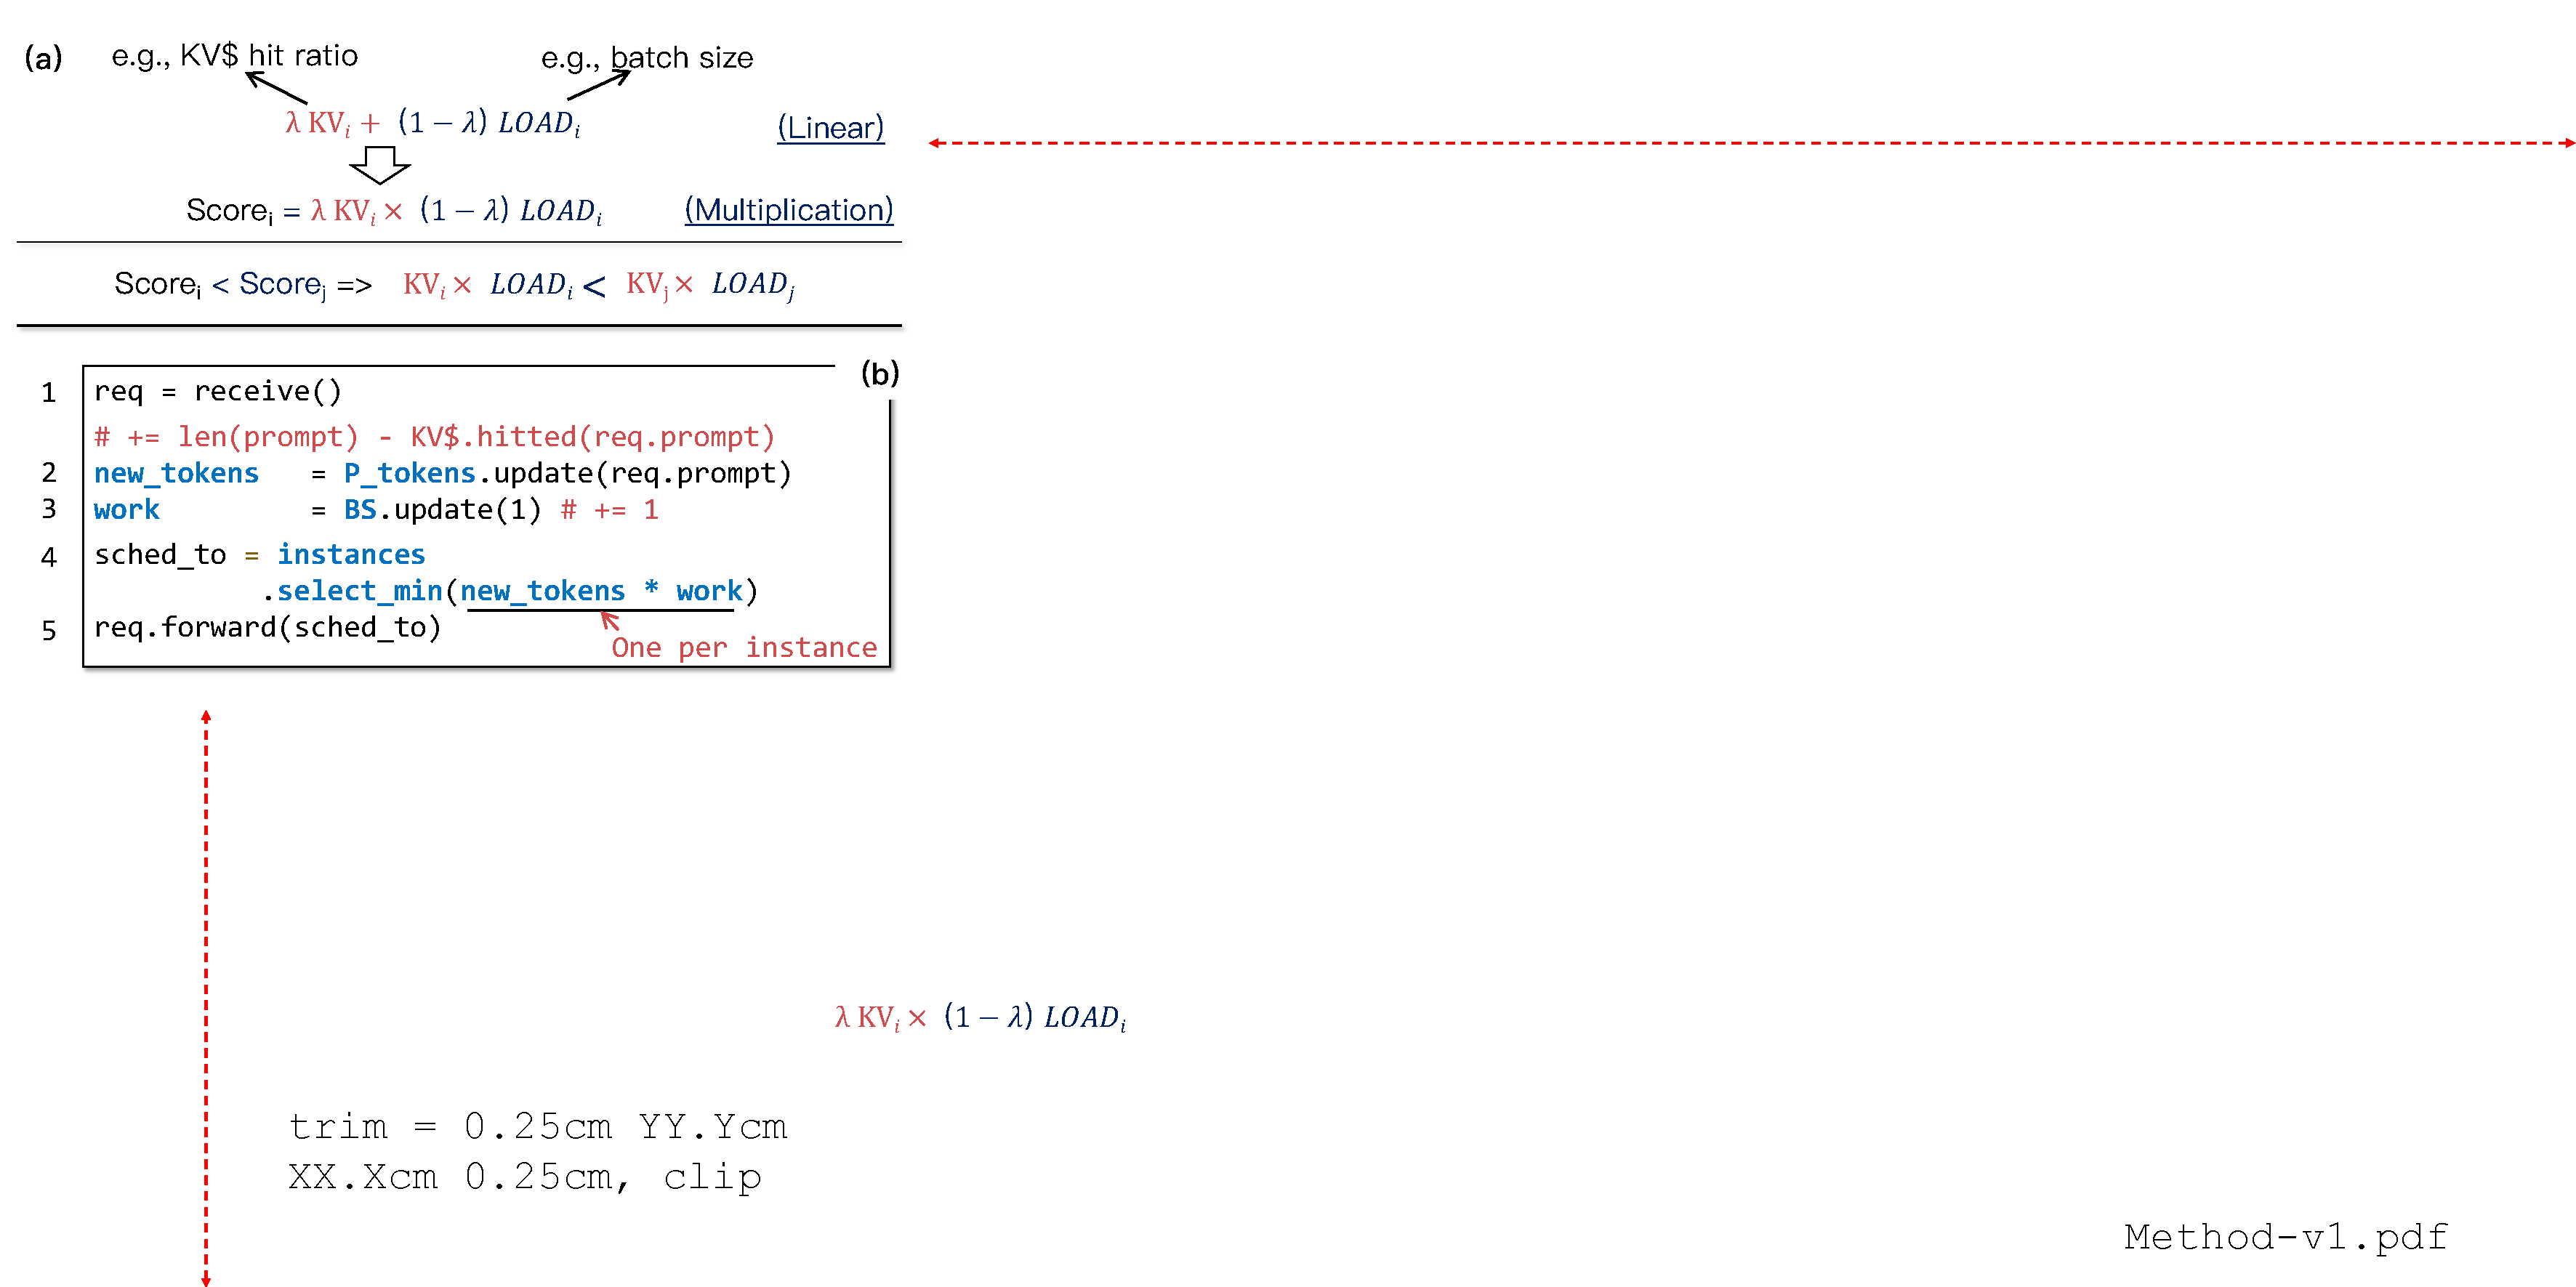
\includegraphics[width=0.95\linewidth, trim=0.25cm 13.5cm 38.4cm 0.25cm, clip]{figs/method-v1.pdf}
        \end{minipage} \\[-1pt]
        \begin{minipage}{1\linewidth}
        \caption{\small{%
    (a) 乘法如何在组合两个指标时避免线性组合所需超参数的示意图；
    以及 (b) 我们调度方法的伪代码。
        }}  
        \label{fig:method}
        \end{minipage} \\[-0pt]
        \end{figure}

\nospacestitle{方法概述（{\fig{fig:method}}）。\,}
我们的方法非常简单：只需将两个精心选择的指标相乘来计算调度分数，
一个用于 {\kvcache} 感知，另一个用于负载均衡，
然后把请求路由到分数最小的实例。
这一做法的基本思想是：
如果两个指标的线性组合有效，那么乘法通常也能以类似方式工作，
同时还具备一个额外优势——无需进行超参数调优，如图 (a) 所示。
两个指标的具体选择——\textbf{P-token}（考虑 {\kvcache} 命中后，若将请求路由到某实例所需的新预填充 token 数）
以及 \textbf{BS}（实例的批大小）——来自我们在 \textsection{\ref{sec:indicators}} 中的细致分析。

为了理解为什么把请求路由到 (P-Tokens \(\times\) BS) 最小的实例能够同时兼顾两个目标，
考虑两个实例 $i$ 和 $j$：
如果把请求路由到实例 $i$ 相比路由到实例 $j$ 能带来更多的 {\kvcache} 命中，
那么实例 $i$ 的 \textbf{P-token} 值就会更低，
除非实例 $i$ 中已经排队了大量预填充请求（这表明出现了工作失衡）。
与此同时，\textbf{BS} 刻画了每个实例上的解码工作负载；
因此，如果实例 $i$ 的批大小显著大于实例 $j$，
乘法分数就很可能会倾向于实例 $j$，从而实现负载均衡。

我们也承认，确实存在一些乘法可能失效的情形：
由于 {\kvcache} 访问极度偏斜，
某一组实例会因为持续拥有很高的 {\kvcache} 命中（即很低的 \textbf{P-token}）而总是被选中，
而这些实例上不断增大的批大小（\textbf{BS}）却不足以抵消如此低的 \textbf{P-token} 值。
正如我们将在 \textsection{\ref{sec:m-analyze}} 中分析的，这类情形在实践中非常罕见，
并且可以事先检测到（从而进行缓解）。

\subsection{指标的选择}
\label{sec:indicators}


\begin{figure}[!t]
        \begin{minipage}{1\linewidth}
        \centering
        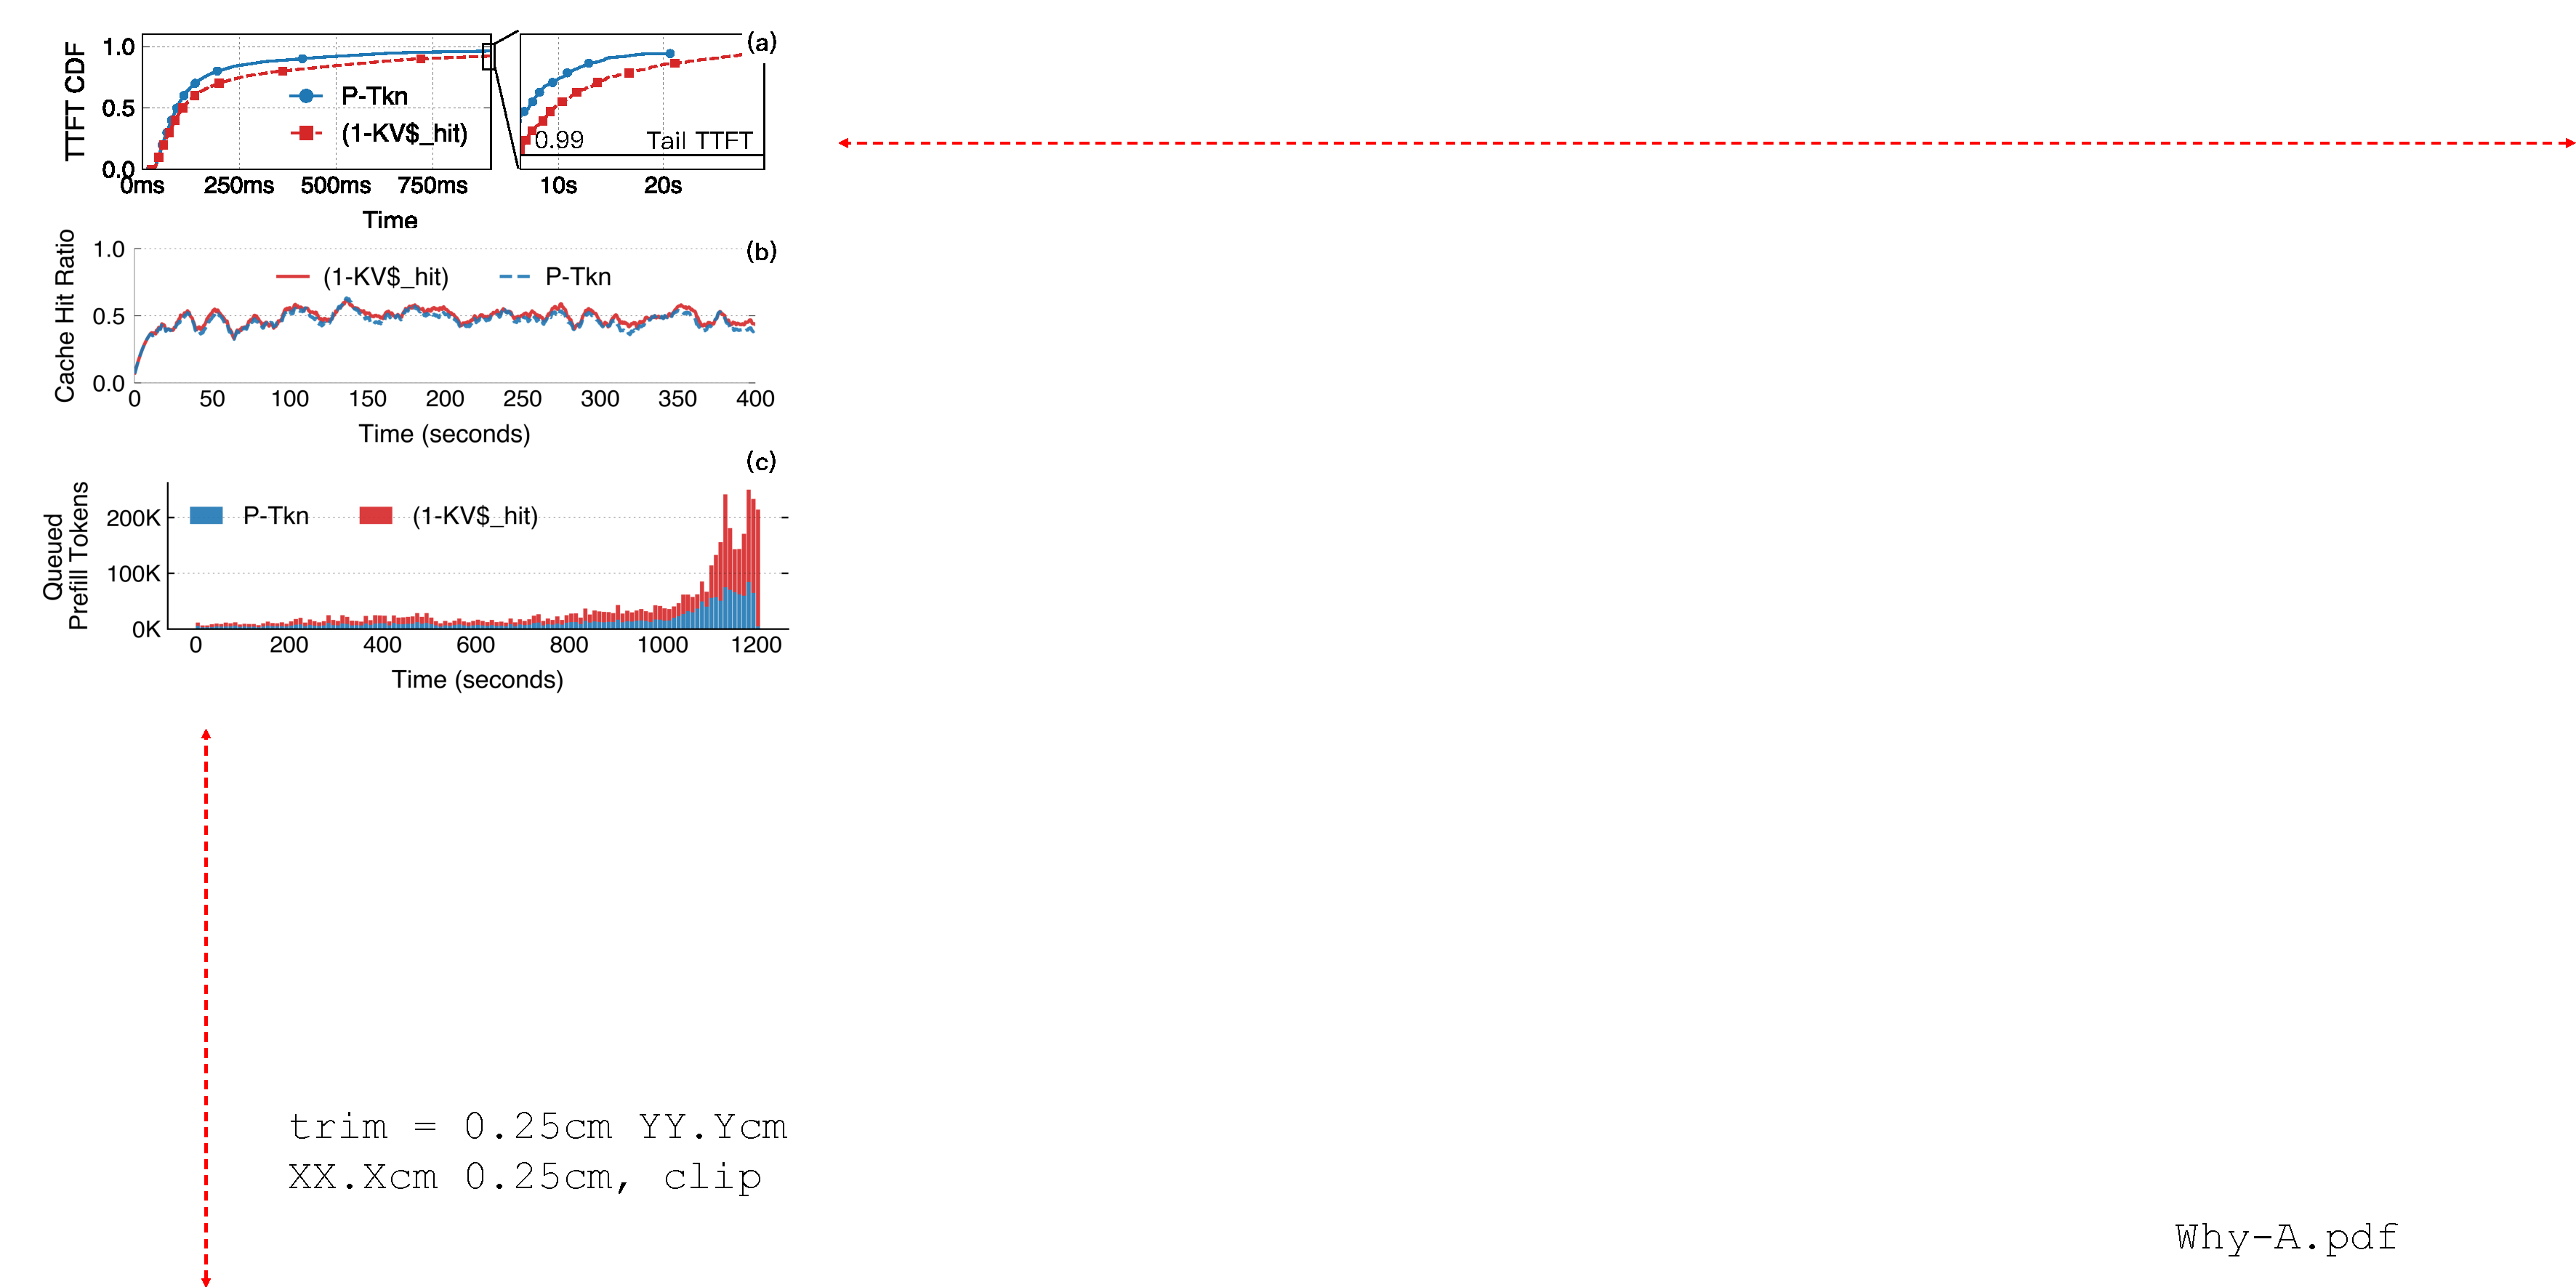
\includegraphics[width=0.99\linewidth, trim=0.25cm 13.1cm 40.5cm 0.25cm, clip]{figs/5-1-select-A-B/why-A.pdf}
        \end{minipage} \\[-1pt]
        \begin{minipage}{1\linewidth}
        \caption{\small{%
    (a) 在 $A \times BS$ 调度中，使用新增预填充 token（P-Tkn）与使用 1-{\kvcache} 命中率（1-KV$_{hit}$）作为 {\kvcache} 感知指标（$A$）的比较；
    (b) {\kvcache} 命中率分析；
    以及 (c) 排队预填充 token 分析。
    该分析基于 Qwen3-30B 模型和 ChatBot(Qwen) 轨迹。
        }}  
        \label{fig:whyA}
        \end{minipage} \\[-0pt]
        \end{figure}

\nospacestitle{{\kvcache} 感知指标（P-token）。\,}
除了 \textbf{P-token} 之外，另一个自然的 {\kvcache} 感知指标是
\textbf{1-{\kvcache} 命中率}，即请求被路由到某实例时的 {\kvcache} 命中率。
Preble~\cite{DBLP:conf/iclr/SrivatsaHAL025} 和 AIGW~\cite{aigw} 等工作都采用了这种做法。
这里取一减，是因为更高的 {\kvcache} 命中率应对应更低的分数，
从而与新增预填充 token 指标的方向保持一致。
我们没有考虑 TTFT 作为指标，因为它需要依赖模拟器的开发，而这并不总是适用。

我们的经验分析表明，使用 \textbf{P-token} 比使用 \textbf{1-{\kvcache} 命中率} 能取得更好的性能。
从 {\fig{fig:whyA}} (a) 可以看到，在负载均衡指标都固定为 \textbf{BS} 的公平比较下，
使用 \textbf{P-token} 能够带来低 14.4\% 的 P50 TTFT 以及低 42.8\% 的 P95 TTFT。
由于篇幅限制，我们这里只报告一个工作负载的结果；
不过这一趋势在所有评估过的工作负载上都一致。

为了理解差异的根源，
{\fig{fig:whyA}} 在 (b) 中进一步拆解了不同方法的 {\kvcache} 命中率，
并在 (c) 中展示了负载均衡状况。
可以看到，两种方法获得的 {\kvcache} 命中率相近，
因此它们都以类似方式实现了 {\kvcache} 感知。
真正的差异在于，使用 \textbf{P-token} 能实现更好的负载均衡，
因为它额外考虑了每个实例上排队等待的预填充 token。
因此，在做调度决策时，即便某些实例有较高的 {\kvcache} 命中率，
路由器也会绕开那些已经排队了大量预填充请求的实例。


\begin{figure}[!t]
        \hspace{-2mm}
        \begin{minipage}{1\linewidth}
        \centering
        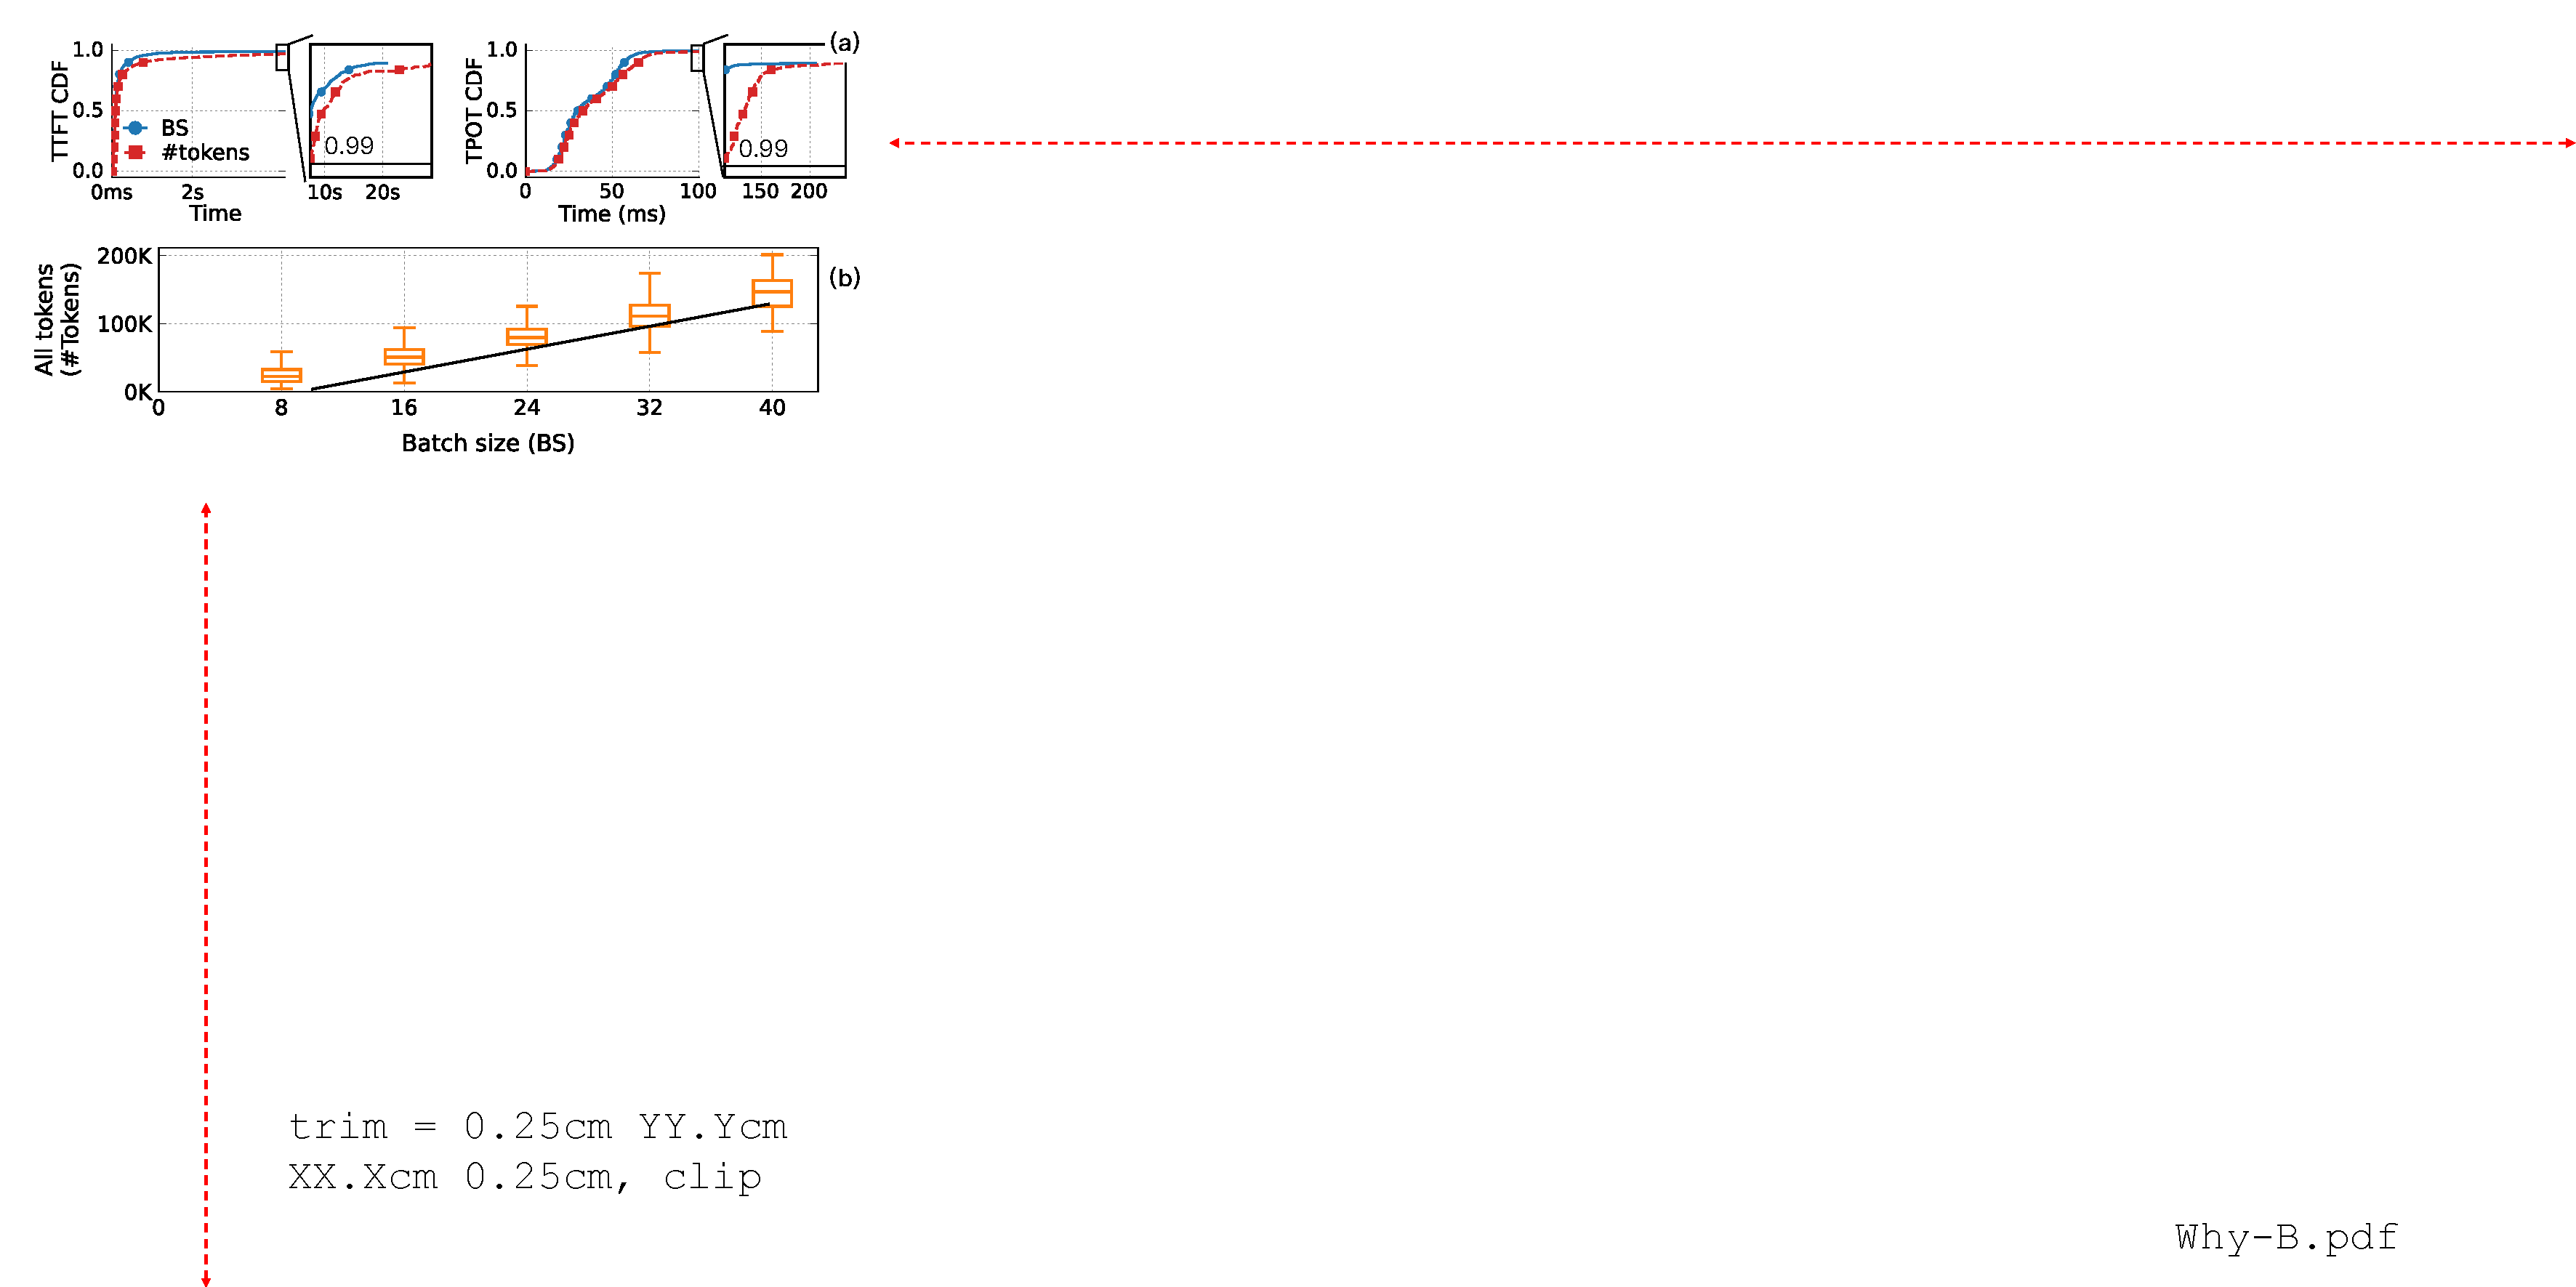
\includegraphics[width=0.99\linewidth, trim=0.25cm 18.5cm 39.5cm 0.25cm, clip]{figs/bs-relation-totaltkns-tbt/why-B.pdf}
        \end{minipage} \\[-2pt]
        \begin{minipage}{1\linewidth}
        \caption{\small{%
    (a) 在 $P$-Tokens \(\times\) $B$ 调度中，使用批大小（BS）与使用总 token 数（\#Tokens）作为负载均衡指标（$B$）的比较。
    (b) 对批大小与总 token 数关系的剖析。
    该分析基于 Qwen3-30B 模型和 ChatBot(Qwen) 轨迹。
        }}  
        \label{fig:whyB}
        \end{minipage} \\[-0pt]
        \end{figure}


\stitle{负载均衡指标（BS）。\,}
除了 \textbf{BS} 外，另一个常见选择是每个实例上的总 token 数（\textbf{\#Tokens}），
ai-Dynamo~\cite{ai-Dynamo}、AIGW~\cite{aigw} 等工作都采用了这一指标。
其理由是，一个请求的总计算成本与其上下文中的 token 数成正比。
然而，我们发现使用 \textbf{BS} 效果更好，
{\fig{fig:whyB}} (a) 展示了这一点，其原因有二。
第一，工作负载可以分为预填充负载与解码负载，而前者已经由我们的 \textbf{P-Tokens} 指标刻画。
因此，我们只需要一个描述解码负载的指标，而这正是 \textbf{BS} 所捕获的内容（我们也尝试过使用 decode batch size，结果类似，因为 \textbf{BS} 主要由解码请求主导）。
第二，\textbf{BS} 更适合作为实例上（解码）工作量的指标，
因为解码时间在不同批大小下更稳定：更大的批大小往往对应更长的解码时间；
但更多的解码 token 并不一定意味着更长的解码时间，
因为在小批次情况下，借助 {\kvcache}，解码可能依然很快~\cite{DBLP:conf/osdi/ZhongLCHZL0024}。
这一点在 {\fig{fig:whyB}} (b) 中得到了说明：
我们在那里刻画了在 Qwen3-30B 上服务 ChatBot(Qwen) 工作负载时，批大小与总 token 数之间的关系。


\subsection{基于乘法调度分数的良性情形与失效情形分析}
\label{sec:m-analyze}

\nospacestitle{概览。\,}
从高层看，只要不存在负载失衡——也就是某些实例过载而其他实例空闲——
那么把请求路由到具有较高 {\kvcache} 命中率（即较低 \textbf{P-token}）的实例总是有利的。
因此，当一组实例即将发生负载失衡，
但这些实例上不断增加的 \textbf{BS} 无法抵消由于较高 {\kvcache} 命中率而带来的 \textbf{P-token} 降低时，
乘法就可能失效；
结果就是请求会持续被路由到这些“即将过载”的实例上，并最终造成失衡。
这类情况会出现在极端的 {\kvcache} 偏斜下：
某一小类请求反复访问一组实例上的同一前缀——我们将这种现象称为 \emph{{\kvcache} 热点}。
我们发现，这种热点在实践中非常少见——至少在本文评估的所有轨迹中都没有出现；
更重要的是，由于其模式非常清晰，我们可以设计探测器在事先将其识别出来。

因此，为了分析乘法方法的失效情形，
我们需要推导出：在给定工作负载模式下，{\kvcache} 热点何时会出现，以及在该情况下增加的批大小为何不足以抵消高 {\kvcache} 命中率所带来的优势。
对于每个工作负载，我们首先按 {\kvcache} 前缀对请求分组，再依据 {\kvcache} 命中率对实例做划分。
随后，对每一个请求类别，我们都可以具体分析工作负载模式、由 {\kvcache} 命中率决定的 P-token 指标，以及批大小指标三者之间的关系。

\stitle{前奏：请求分组与实例划分。\,}
首先，我们将所有请求划分为一组类别
\(\mathcal{C}\)，其中每个 \(c\!\in\!\mathcal{C}\) 对应一类共享相同 {\kvcache} 前缀的请求。
在实践中，一个类别大致对应某个应用或某个用户：它们的请求共享相同的系统提示词，并且往往拥有相似的对话历史~\cite{10.5555/3768039.3768067}。
对一个固定类别 \(c\)，我们考虑一个累积时间窗
\((t, t+\textit{window})\)，并用 \(x\) 表示在该时间窗内到达集群的所有请求中属于类别 \(c\) 的比例；
剩余比例则记作 \(\bar{x} = 1-x\)。

对于每个类别 \(c\)，我们再把集群划分为两组实例：
\(M\) 和 \(\bar{M}\)。
\(M\) 包含当前缓存中保存了类别 \(c\) 前缀、即存在 {\kvcache} 命中的实例；
而 \(\bar{M}\) 则包含所有其他实例。

\stitle{请求类别对批大小的影响。\,}
设 \(\text{QPS}\) 为集群总请求率，
并令 \(t\) 表示可能导致失衡的类别 \(c\) 请求到达的时刻。
我们记在时刻 \(t\) 之前、系统处于平衡状态时，每个实例的平均批大小为 \(BS_0\)。
同时，用 \(BS_{t}\) 和 \(\overline{BS}_{t}\) 分别表示在区间 \((t, t+\textit{window})\) 内，\(M\) 与 \(\bar{M}\) 中实例的期望批大小。
我们考虑一种极端情况：由于极高的 {\kvcache} 命中率，所有属于类别 \(c\) 的请求都会被路由到 \(M\)；
因为如果其中一部分请求被路由到 \(\overline{M}\)，那么热点本身就已经通过把流量分散到更多机器上而得到缓解。
因此，我们可以得到一个近似表达式，用来刻画“潜在过载实例”的批大小与“非过载实例”的批大小之比：

\begin{equation}
\frac{BS_{t}}{\overline{BS}_{t}}
  = \frac{
      BS_0 + \left( x \cdot \text{QPS}\right) / |M| \cdot t
    }{
      BS_0 + \left( \bar{x} \cdot \text{QPS}\right) / |\overline{M}| \cdot t
    }.
\label{eq:bs-ratio-exact}
\end{equation}
主导项
\(\left( x \cdot \text{QPS}\right) / |M| \cdot t\) 对应的是
类别 \(c\) 的请求被路由到缓存了其前缀的实例上的数量；
而 \(\left( \bar{x} \cdot \text{QPS}\right) / |\overline{M}| \cdot t\) 则对应其余所有请求被路由到剩余实例上的情况。

\stitle{分析：良性情形，以及它们是否常见？\,}
只要疑似热点实例的批大小没有高于其他实例，
那么把请求路由到这些实例显然是有益的，
因为这种决策能够提升 {\kvcache} 命中率，同时不会造成负载失衡。
而我们的乘法分数正会忠实地做出这样的选择，
因此这些情形对我们的方法而言属于“良性情形”。
剩下的问题是：这种情形在实践中常见吗？
幸运的是，基于方程~\ref{eq:bs-ratio-exact} 所建立的“工作负载—批大小”关系，
我们可以通过追踪不同轨迹中的两个量
\(\frac{x}{\bar{x}}\) 和 \(\frac{|M|}{|\overline{M}|}\)，对其出现频率进行经验分析。
这里我们在每个时间窗（1 分钟）中采样 {\kvcache} 命中率最高的请求类别。

\begin{figure}[!t]
          \vspace{1mm}
          \begin{minipage}{1\linewidth}
          \centering
          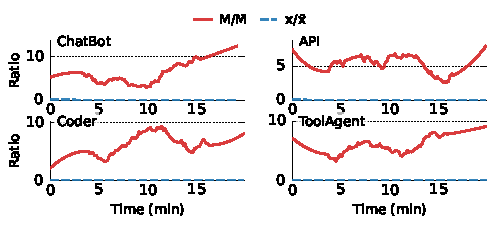
\includegraphics[width=0.98\linewidth ]{figs/5-3-detector/detector-allinone.pdf}
          \end{minipage} \\[1pt]
          \begin{minipage}{1\linewidth}
          \caption{\small{%
不同轨迹中乘法分数相关因素的经验观测。
如果 $\frac{x}{\bar{x}} \leq \frac{|M|}{|\overline{M}|}$，则不会出现由 {\kvcache} 热点导致的负载失衡，
因此我们的乘法方法能够在保持 {\kvcache} 感知的同时有效实现负载均衡。
          }}  
          \label{fig:detector}
          \end{minipage} \\[-0pt]
          \end{figure}

\begin{equation}
\frac{x}{\bar{x}}
\leq
\frac{|M|}{|\overline{M}|}
\label{eq:consensus-1}
\end{equation}


{\fig{fig:detector}} 表明，本文研究的所有轨迹——它们能够代表真实 LLM 服务场景——对于我们的方法都属于良性情形，
因为疑似热点实例的期望批大小并不大于其他实例。
这一点可以作如下解释。
根据 {\fig{fig:detector}}，对所有轨迹我们都能观察到由方程~\ref{eq:consensus-1} 概括的关系。

\begin{equation}
\frac{x}{|M|}
\leq
\frac{\bar{x}}{|\overline{M}|}
\label{eq:consensus-2}
\end{equation}

\noindent
对方程进行整理后即可得到方程~\ref{eq:consensus-2}。
将其代入方程~\ref{eq:bs-ratio-exact}，
我们便得到：{\kvcache} 热点实例的期望批大小小于其他实例。

\stitle{分析：失效情形，以及我们的两阶段探测器。\,}
根据前述分析可知，如果方程~\ref{eq:consensus-1} 不成立，即
\[ \frac{x}{\bar{x}} > \frac{|M|}{|\overline{M}|}  \]，
那么就存在 {\kvcache} 热点导致负载失衡、从而破坏我们乘法方法的可能性。
这为失效情形提供了一个仅依赖工作负载模式与 {\kvcache} 状态的清晰探测信号，
因此我们可以在真正做出调度决策前，就开发一个探测器去捕获这类潜在失效。

具体而言，对于每个请求类别，我们实时统计两个量 \(\frac{x}{\bar{x}}\) 与 \(\frac{|M|}{|\overline{M}|}\)。
如果观察到方程~\ref{eq:consensus-1} 不成立，
我们就触发第一阶段告警，并把疑似实例（\(M\)）从候选路由目标中临时过滤掉。
为了避免追踪过多请求类别带来的开销，我们只跟踪那些 {\kvcache} 命中率最高的请求。

单阶段探测器的问题在于：
即使方程~\ref{eq:consensus-1} 不成立，把请求路由到拥有高 {\kvcache} 命中的疑似实例，有时仍然是值得的，
只要我们不会把过多请求连续发往这些热点实例。
因此，我们进一步加入第二阶段：
并不在第一阶段告警时立即过滤，而是延迟到我们观察到某个类别的请求连续多次被路由到热点实例之后再采取动作；
因为连续的路由决策往往意味着，疑似实例上批大小的增加已经不足以抵消其高 {\kvcache} 命中率所带来的优势。

\begin{equation}
  \text{P-token}_m \times BS_m \leq \text{P-token}_{\bar{m}} \times BS_{\bar{m}}
  \label{eq:m-score}
\end{equation}

具体做法是：在第一阶段触发告警后，我们继续跟踪该类别请求的新增预填充 token；
如果我们观察到，超过 \(2 \times M\) 个连续请求在某个疑似热点实例（$m$）上的乘法分数（方程~\ref{eq:m-score}）
都小于其在其他实例（$\bar{m}$）上的分数，
那么就触发第二阶段告警，并把这些疑似实例从路由目标中过滤掉。
